

A partir de la secuencia de puntos rotada, suavizada y re-muestreada $\rv_i$ se calcula la característica que se utilizará para reconocer los gestos. La misma es el denominado \textbf{vector de primeras diferencias}; este vector contiene las direcciones entre cada par de posiciones consecutivas del gesto. Por ejemplo, el elemento 1 del vector de primeras diferencias contiene la dirección para llegar desde la posición 1 a la posición 2 del gesto.

Las direcciones de este vector a su vez se escalan a norma 1 para remover toda la información de velocidad y escala contenida en la secuencia de posiciones originales. 

\image{features}{0.8}{Cálculo de características a partir de un ejemplar de gesto normalizado.}

El \textbf{vector de primeras diferencias normalizado} del ejemplar $i$, $\xv_i$, está dado entonces por:

\ma{
\xv_i[j]= \frac{\rv_i[j+1]-\rv_i[j]}{||\rv_i[j+1]-\rv_i[j]||}, \qquad j=1 \dots n-1,  \qquad \xv_i[j] \in \reals^3 }

Este vector será la característica para el gesto, y cada uno de sus elementos representa la dirección relativa entre las posiciones consecutivas del mismo. A la función característica que lo calcula se la denominará $\phi_d$. El vector de primeras diferencias, sin normalizar, da una representación equivalente invariante a la traslación. Al normalizar, se remueve toda la información de velocidad y escala contenida en la norma de cada vector de dirección, tornando la característica invariante a la velocidad y escala. 

Es importante notar que sin el re-muestreo esta normalización dejaría todavía una cantidad considerable de información de velocidad en la señal, debido a que la cantidad de puntos de muestreo en los segmentos (interpretando la palabra en el sentido de la longitud de arco) donde el usuario realizar el gesto a altas velocidades es más bajo que en aquellos segmentos en donde la mano se mueve más lentamente. Es decir, a mayor velocidad, menor densidad de puntos de muestreo y viceversa. 

Por último, la característica es en cierto modo equivalente a la función \textit{ángulo-tangente} \cite{Kindratenko:2003} para describir formas de objetos, y por eso desde esa equivalencia también se puede argumentar que cumple las propiedades de invariancia a la escala, traslación y velocidad.

%Como una alternativa a los vectores dirección, empleamos también los ángulos de la representación esférica de los vectores dirección, obteniendo una representación $\ve{a_i}$, donde $\ve{a_i}[j]=(\theta,\phi)_j \in \reals^2$.  La coordenada $z$ de la representación esférica se obvia debido a que es siempre $1$ a consecuencia de la normalización previa, y reescalamos los ángulos de manera que  $\theta,\phi \in [-1,1]$.

%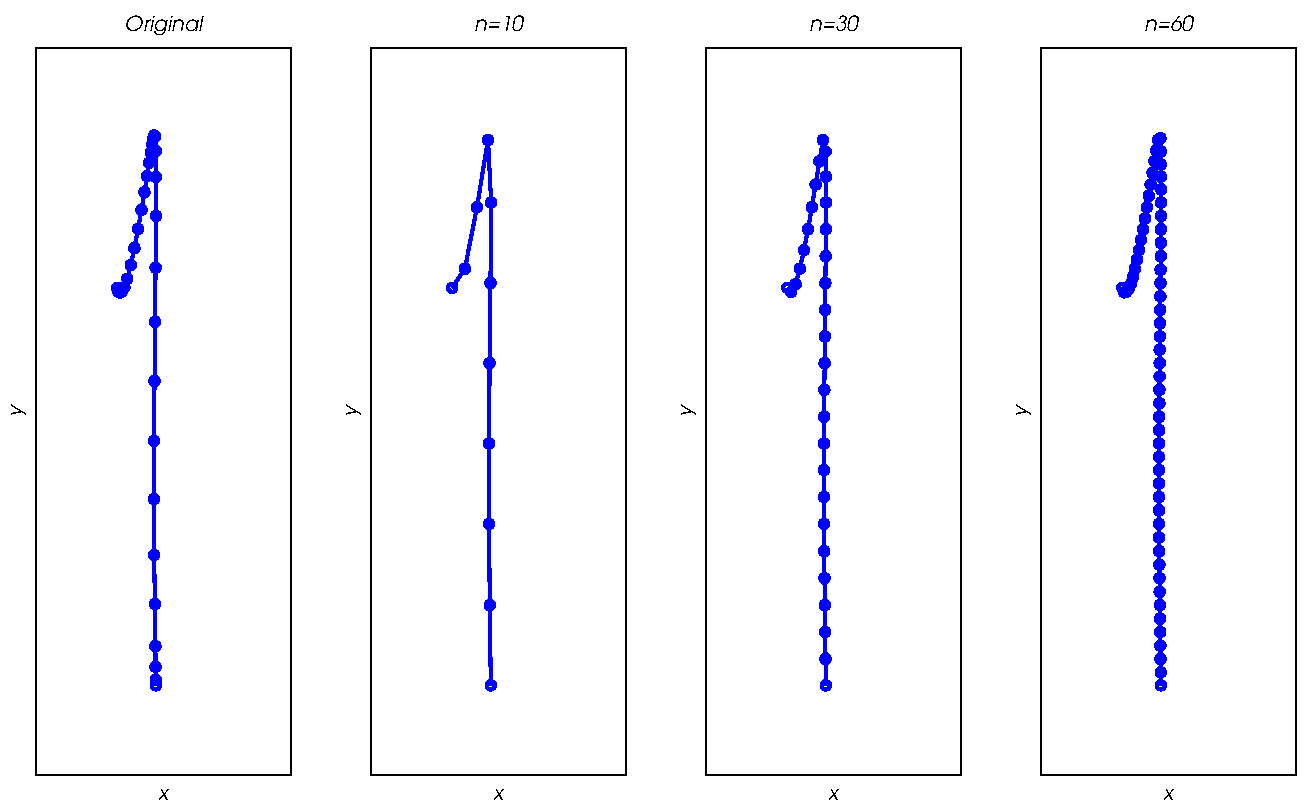
\includegraphics[scale = 0.2]{img/direction}

%Dada la naturaleza periódica de la representación con ángulos, en todas las diferencias entre ángulos calculadas para los algoritmos de clasificación utilizamos la función $ d(\alpha,\beta) = min(|\alpha-\beta|, 2- |\alpha-\beta|)$.

%Aunque ambas características son isomorfas y tienen las mismas propiedades deseables ( invariancia a la escala, traslación y velocidad \cite{Kindratenko:2003}), producen resultados ligeramente distintos en nuestros experimentos. En las siguientes secciones nos referirmos a las características calculadas a partir de un ejemplar de gesto como $\xv$, donde $\xv[j] \in \reals^d$ puede referirse a cualquiera de las dos características (con $d=2$ para ángulos y $d=3$ para direcciones cartesianas). 


\subsection{Versiones discretas de las propiedades de los gestos}

Previamente se definió un modelo de gestos donde un gesto es una trayectoria continua y hay una relación de equivalencia entre gestos con propiedades deseables. Como los ejemplares son una secuencia de posiciones discretas, se necesita una versión discreta de dichas propiedades, aplicables a la representación que se utiliza en los algoritmos de clasificación. La principal diferencia entre ambas es la función de correspondencia entre gestos, ya que de todas maneras se busca una matriz de rotación $\roti$, y constantes de traslación y escala $a$ y $c$. Recordando la definición para el caso continuo:


\equivalencia{ m}{
 & \existsroti, \existsb, \existsa
\\ & c(l) \eequiv a (\roti c'(l))+b
}

Se busca aproximar dicha definición en el caso concreto. Para ello, el re-muestreo de un gesto da una representación de sus posiciones $\ve{r}$ que es uniforme en la longitud total de arco del gesto, y que dado un $n$ lo suficientemente grande, aproxima con error arbitrario a la representación continua.  Entonces, se define la equivalencia en el caso discreto simplemente como:

\tci{ \sv &\equiv_m \sv' }
{& \existsroti,  \existsb,  \existsa \\ 
& \sv[j] \eequiv  a (\roti \sv'[j])+b, \; \range{j}{1}{n}  }


Como el espacio de búsqueda de dicha transformación es muy grande, se debe encontrar una equivalencia entre características dadas por $ \fdef{\phi}{\ddp}{\mathcal{F}}$, donde $\mathcal{F}$ es el espacio de características, de manera que si $ \phi(\sv) \eequiv \phi(\sv') \tn \xv \equiv_m \xv'$. Es decir, equivalencia en el espacio de las características implica  equivalencia $\equiv_m$. 

En esta tesina, se llamará  $\phi_d$ a la función característica que dado un ejemplar de gesto realiza la normalización, incluyendo rotación, suavizado y re-muestreo, y el cálculo de la primera diferencia con norma 1; es decir, $\xv_i=\phi_d(\sv_i)$. 

Debido a la corrección de la rotación, en donde siempre se ubica el cuerpo en cierto sentido, $\phi_d$ es invariante a la rotación. No es invariante a otras rotaciones, ya sean en otras direcciones o de las manos en sí.

Gracias al re-muestreo y la parametrización por longitud de arco, $\phi_d$ es invariante a la velocidad con la cual fue realizado el gesto, y permite que cada $\xv[j]$ represente siempre la misma parte del gesto, aunque sea de forma aproximada.

El cálculo de la primera diferencia provee invariancia a la traslación, ya que no importan las posiciones absolutas sino las direcciones entre ellas. Llevar dichas diferencias a norma 1 otorga invariancia a la escala, ya que así no influye la distancia absoluta entre posiciones contiguas, sino su dirección solamente.

El vector característico $\xv$ es invariante, como se deseaba, a la rotación, traslación, velocidad y escala.

Por último, se define la propiedad de invariancia al punto de comienzo para gestos cerrados discretos, para algún clasificador que pueda implementarla.

En el caso discreto, los gestos cerrados son aquellos para los cuales $\sv[1] = \sv[n]$. Entonces, una característica $\phi$ es invariante a la posición de comienzo si:

\ma{
&\phi(\sv) =\phi( shift(\sv,k)), \quad k=1..n-1  \\
&\text{donde} \\
& \quad shift(\xv,k)=( x_{ (k) \% (n+1)}, x_{ (k+1) \% (n+1)},\dots, x_{ (n+k) \% (n+1)} ) \\
& \quad \text{y \% es el operador \textit{modulo}}
}

La característica $\phi_d$ que se desarrolló en la sección anterior no es invariante al punto de comienzo, debido a que claramente un \textit{shift} de los puntos del gesto causa un \textit{shift} en la característica calculada. El clasificador CNC que se describe en el  capítulo \ref{chap:resultados} \textit{si} provee invariancia al punto de comienzo realizando una transformación posterior a las características obtenidas con $\phi_d$, a costa de perder información sobre la \textit{secuencia} de las direcciones.

En conclusión, se ha definido una característica $\phi$ para una secuencia de puntos 3D $\sv$, y establecido que es invariante a la rotación, traslación, velocidad y escala (o sea  $ \xv \eequiv \xv \tn \sv \equiv_m \sv'$)  propiedades de utilidad para el reconocimiento de gestos.